\documentclass{standalone}
\usepackage{tikz}
\usepackage{kpfonts}
\usepackage{xcolor-solarized}
\usetikzlibrary{decorations.pathmorphing}
\usetikzlibrary{positioning}
\usetikzlibrary{shapes.misc}
\usetikzlibrary{shapes.geometric}
\usetikzlibrary{shapes.symbols}
\usetikzlibrary{arrows}
\usetikzlibrary{fit}
\usetikzlibrary{backgrounds}

\begin{document}
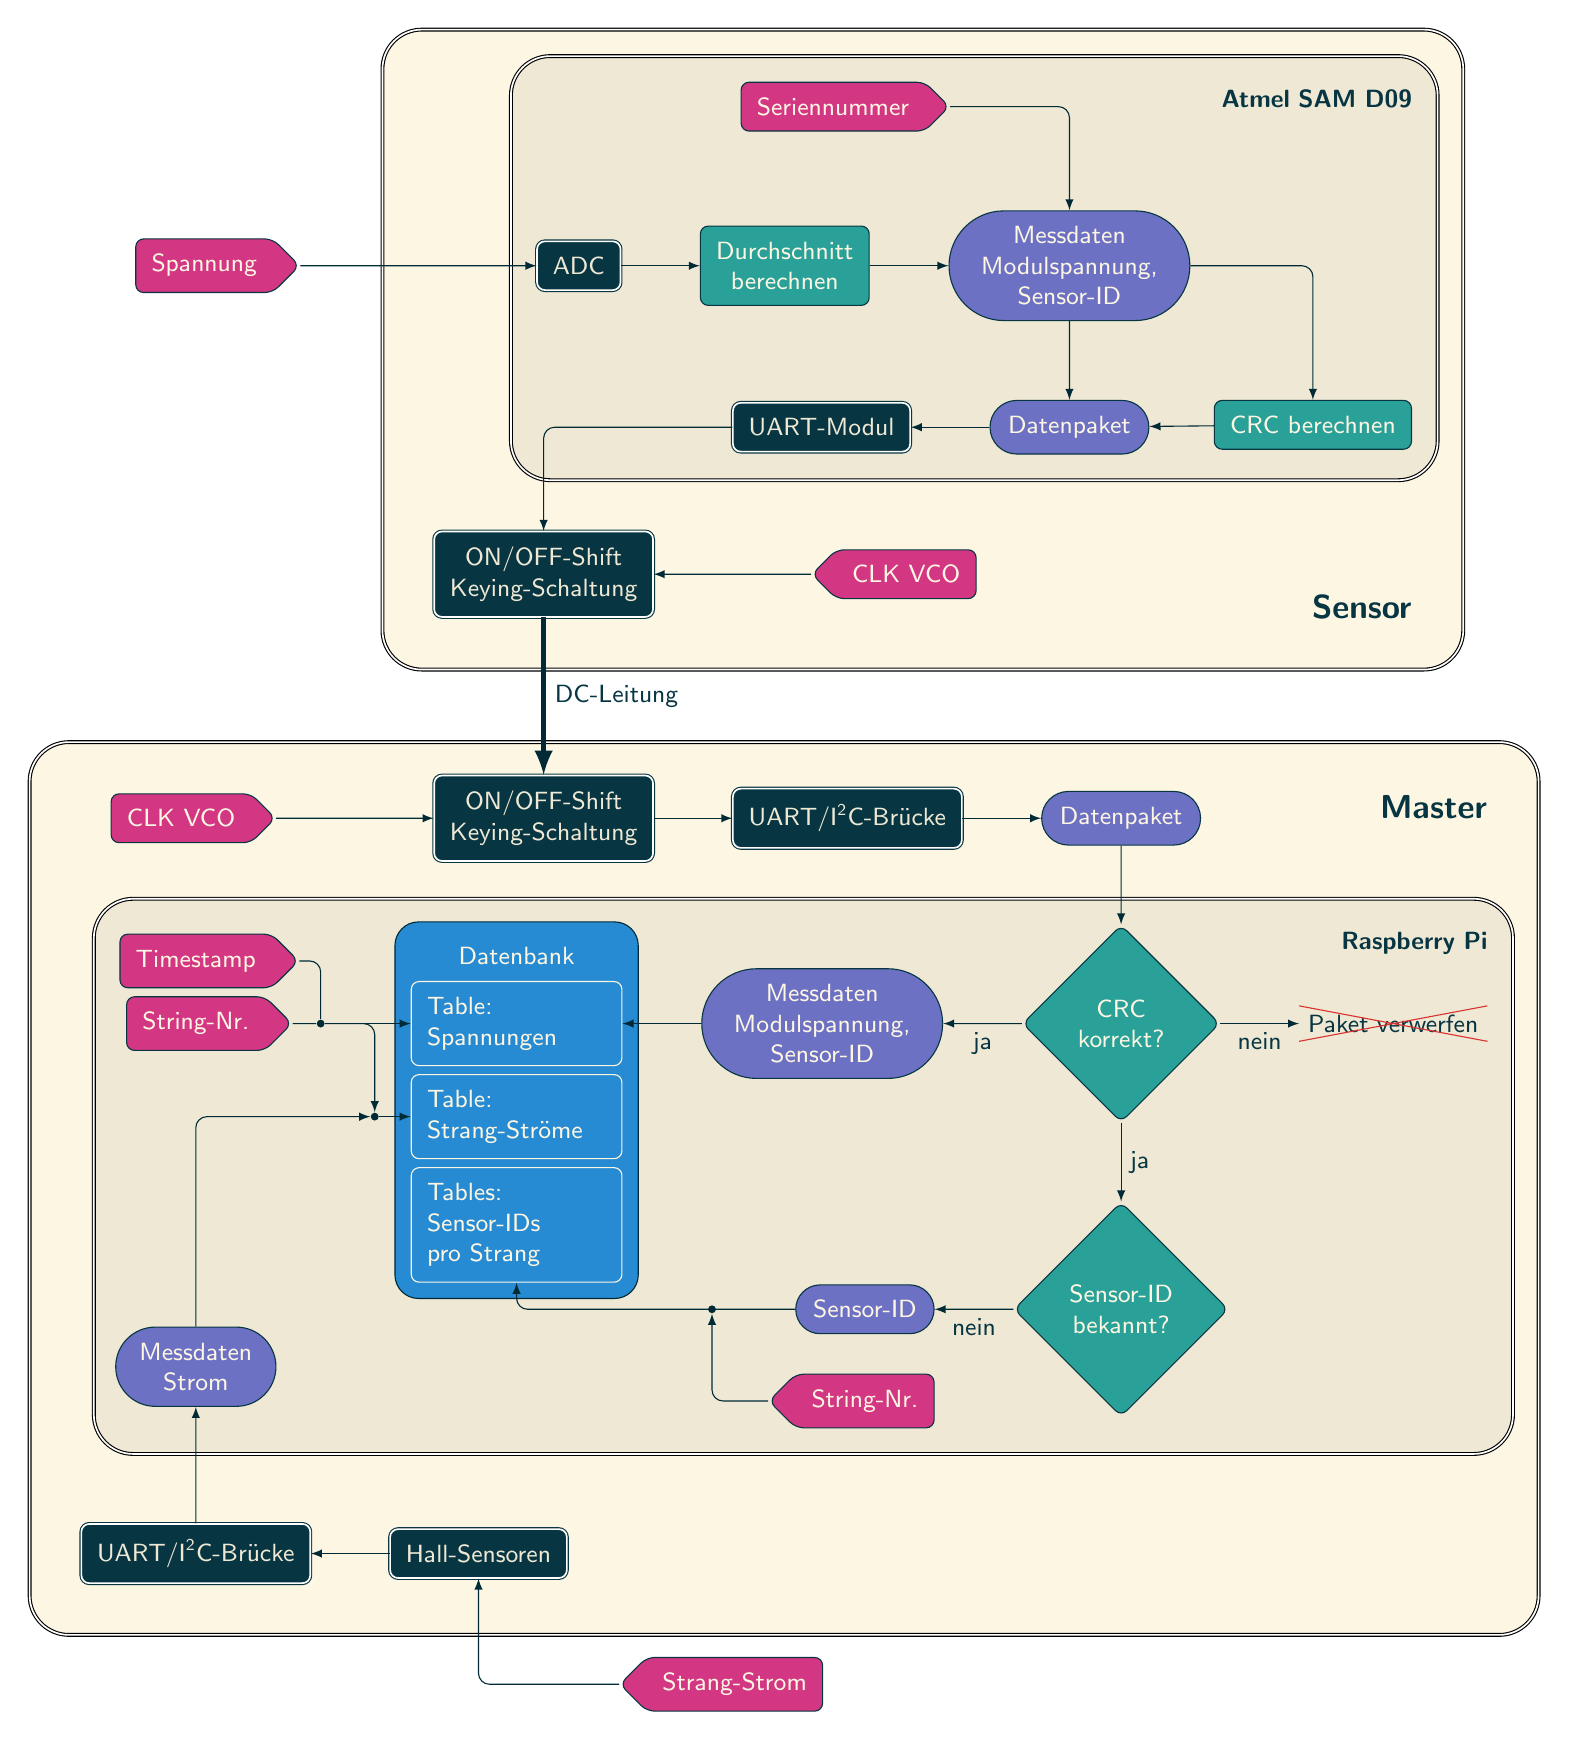
\begin{tikzpicture}[%
        align=center,
        text=solarized-base02,
        draw=solarized-base02,
    ]
    \small
    \sffamily

    \begin{scope}[
        every node/.style = draw,
        terminal/.append style={
            rounded rectangle,
            fill=solarized-violet,
            text=solarized-base3,
            inner sep=2mm,
        }, % data packages
        sign/.style={
            inner sep=2mm,
            rounded corners=1mm,
            fill=solarized-magenta,
            text=solarized-base3,
        },         % custom signal style
        circ/.style={
            inner sep=2mm,
            rounded corners=1mm,
            double,
            fill=solarized-base02,
            draw=solarized-base02,
            text=solarized-base2,
        }, % circuitry
        proc/.style={
            inner sep=2mm,
            rounded corners=1mm,
            fill=solarized-cyan,
            text=solarized-base3,
        },       % process/activity
        stor/.style={
            fill=cyan!30
        },         % storage
        dbtable/.style={
            text=solarized-base3,
            draw=solarized-base3,
            rounded corners=1mm,
            inner sep=2mm,
        } % database tables
    ]
        \node (voltage) [
            sign,
            signal,
            signal to=east
        ] at (20mm,-33mm) {Spannung};

        % uC on Sensor
        \node (ADCVolt) [
            circ,
            right=30mm of voltage
        ] {ADC};
        \node (avg) [
            proc,
            right=of ADCVolt,
            align=center
        ] {Durchschnitt\\berechnen};
        \node (data) [
            terminal,
            right=of avg,
            align=center
        ] {Messdaten\\Modulspannung,\\Sensor-ID};
        \node (id) [
            sign,
            signal,
            signal to=east,
            above left=of data
        ] {Seriennummer};
        \node (crc) [
            proc,
            below right=of data
        ] {CRC berechnen};
        \node (package) [
            terminal,
            below=of data
        ] {Datenpaket};
        \node (uart) [
            circ,
            left=of package
        ] {UART-Modul};

        \node (oosk1)[
            circ,
            below left=of uart,
            align=center
        ] {ON/OFF-Shift \\Keying-Schaltung};
        \node (clk1) [
            sign,
            signal,
            signal to=west,
            right=2cm of oosk1
        ] {CLK VCO};
        \node (oosk2) [
            circ,
            below=20mm of oosk1,
            align=center
        ] {ON/OFF-Shift \\Keying-Schaltung};
        \node (clk2) [
            sign,
            signal,
            signal to=east,
            left=2cm of oosk2
        ] {CLK VCO};
        \node (bridge) [
            circ,
            right=of oosk2
        ] {UART/I\textsuperscript{2}C-Br\"ucke};
        \node (package2) [
            terminal,
            right=of bridge
        ] {Datenpaket};

        % Raspi
        \node (crc2) [
            proc,
            align=center,
            diamond,
            below=of package2
        ] {CRC\\korrekt?};
        \node (discard) [
            draw=solarized-red,
            cross out,
            right=of crc2
        ] {Paket verwerfen};
        \node (data2) [
            terminal,
            left=of crc2,
            align=center
        ] {Messdaten\\Modulspannung,\\Sensor-ID};
        \node (dbVolts) [
            dbtable,
            left=of data2,
            text width=7em,
            align=left,
            minimum width=7.5em
        ] {Table:\\ Spannungen\\};
        \node (dbCurr) [
            dbtable,
            below=1mm of dbVolts,
            text width=7em,
            align=left,
            minimum width=7.5em
        ] {Table:\\ Strang-Str\"ome\\};
        \node (dbIDs) [
            dbtable,
            below=1mm of dbCurr,
            text width=7em,
            align=left,
            minimum width=7.5em
        ] {Tables:\\ Sensor-IDs \\ pro Strang};

        \node (newID) [
            proc,
            align=center,
            diamond,
            below=of crc2] {Sensor-ID\\bekannt?};
        \node (sensorID)  [
            terminal,
            left=of newID] {Sensor-ID};
        \node (stringNr2) [
            sign,
            signal,
            signal to=west,
            below=5mm of sensorID
        ] {String-Nr.};

        \node (stringNr) [
            sign,
            signal,
            signal to=east,
            left=15mm of dbVolts
        ] {String-Nr.};
        \node (timestamp) [
            sign,
            signal,
            signal to=east,
            above=1mm of stringNr
        ] {Timestamp};

        \node (dataCurr) [
            terminal,
            below=35mm of stringNr,
            align=center
        ] {Messdaten\\Strom};

        \node (bridge2) [
            circ,
            below=60mm of stringNr
        ] {UART/I\textsuperscript{2}C-Br\"ucke};
        \node (hall) [
            circ,
            right=of bridge2
        ] {Hall-Sensoren};
        \node (current) [
            sign,
            signal,
            signal to=west,
            below right=of hall
        ] {Strang-Strom};
    \end{scope}

    \begin{scope}
        % Need to have this inside  a separate scope so that
        % its border does not get drawn.
        \node (db)        [
            text=solarized-base3,
            above=1mm of dbVolts,
            align=left
        ] {Datenbank};
        \node (dbSignals) [
            circle,
            inner sep=1pt,
            fill=solarized-base03,
            right=3mm of stringNr
        ] { };
        \node (dbSignals2) [
            circle,
            inner sep=1pt,
            fill=solarized-base03,
            left=4mm of dbCurr] { };
        \node (dbSignals3) [
            circle,
            inner sep=1pt,
            fill=solarized-base03,
            left=of sensorID
        ] { };
    \end{scope}

    \begin{scope}[on background layer]
        \node (SENSOR) [%
            draw,
            double,
            rounded corners=5mm,
            fill=solarized-base3,
            inner sep=2em,
            fit=(ADCVolt) (avg) (data) (id) (crc) (package) (uart) (oosk1) (clk1),
            align=left,
            text height=21em,
            align=right,
        ] {\large{\textbf{Sensor}}};
        \node (uCSensor) [%
            draw,
            double,
            rounded corners=5mm,
            fill=solarized-base2,
            inner sep=1em,
            fit=(ADCVolt) (avg) (data) (id) (crc) (package) (uart),
            align=right,
            text height=1em,
        ] {\textbf{Atmel SAM D09}};
        \node (MASTER) [%
            draw,
            double,
            rounded corners=5mm,
            fill=solarized-base3,
            inner sep=2em,
            fit=(clk2) (bridge2) (hall) (stringNr) (timestamp) (crc2) (newID) (discard) (stringNr2),
            align=right,
            text height=1em,
        ] {\large{\textbf{Master}}};
        \node (rasPi) [%
            draw,
            double,
            rounded corners=5mm,
            fill=solarized-base2,
            inner sep=1em,
            fit=(stringNr) (timestamp) (crc2) (newID) (discard) (stringNr2),
            align=right,
            text height=1em,
        ] {\textbf{Raspberry Pi}};
        \node (database) [%
            draw=solarized-base03,
            rounded corners=3mm,
            inner sep=2mm,
            fill=solarized-blue,
            fit=(dbVolts) (dbCurr) (dbIDs) (db),
        ] { };
    \end{scope}


    \begin{scope}[
        rounded corners,
        every path/.append style={draw=solarized-base03,},
    ]
        \draw[-latex] (voltage) -- (ADCVolt);
        \draw[-latex] (ADCVolt) -- (avg);
        \draw[-latex] (id) -| (data);
        \draw[-latex] (avg) -- (data);
        \draw[-latex] (data) -| (crc);
        \draw[-latex] (crc) -- (package);
        \draw[-latex] (data) -- (package);
        \draw[-latex] (package) -- (uart);
        \draw[-latex] (uart) -| (oosk1);
        \draw[-latex] (clk1) -- (oosk1);
        \draw[-latex] (clk2) -- (oosk2);
        \draw[line width=2pt,-latex] (oosk1) --  node[midway, anchor = west] {DC-Leitung} (oosk2);
        \draw[-latex] (oosk2) -- (bridge);
        \draw[-latex] (bridge) -- (package2);
        \draw[-latex] (package2) -- (crc2);
        \draw[-latex] (crc2) -- node[anchor=north] {nein} (discard);
        \draw[-latex] (crc2) -- node[anchor=north] {ja} (data2);
        \draw[-latex] (data2) -- (dbVolts);
        \draw[-] (stringNr) -- (dbSignals);
        \draw[-] (timestamp) -| (dbSignals);
        \draw[-latex] (dbSignals) -- (dbVolts);
        \draw[-latex] (dbSignals) -| (dbSignals2);
        \draw[-latex] (dbSignals2) -- (dbCurr);
        \draw[-latex] (crc2) -- node[anchor=west,align=right] {ja} (newID);
        \draw[-latex] (newID) -- node[anchor=north] {nein} (sensorID);
        \draw[-latex] (sensorID) -| (dbIDs);
        \draw[-latex] (stringNr2) -| (dbSignals3);
        \draw[-latex] (current) -| (hall);
        \draw[-latex] (hall) -- (bridge2);
        \draw[-latex] (bridge2) -- (dataCurr);
        \draw[-latex] (dataCurr) |- (dbSignals2);
    \end{scope}

\end{tikzpicture}
\end{document}
